\section{Performance of Scatter-Based Convolution Compared to cuDNN Convolutions} \label{appendix:compareCUDNN}

In the single-rotation case, the rotation-invariant convolution reduces to a standard convolution. We evaluate our scatter-based convolution (single orientation) through a series of experiments and benchmark it against NVIDIA’s cuDNN convolution library, which is widely used in deep-learning applications \cite{cuDNNsdk}. In our implementation, the fastest cuDNN kernel is automatically selected by the cuDNN autotuner.
The GPU used for evaluation is NVIDIA GeForce RTX 3080 Ti with 16GB video memory. The version of CUDA 12.3 and cuDNN 8.9.6.50 are installed in a Windows 10 system. 

\vspace{0.4cm}  % Add vertical space here
\centerline{
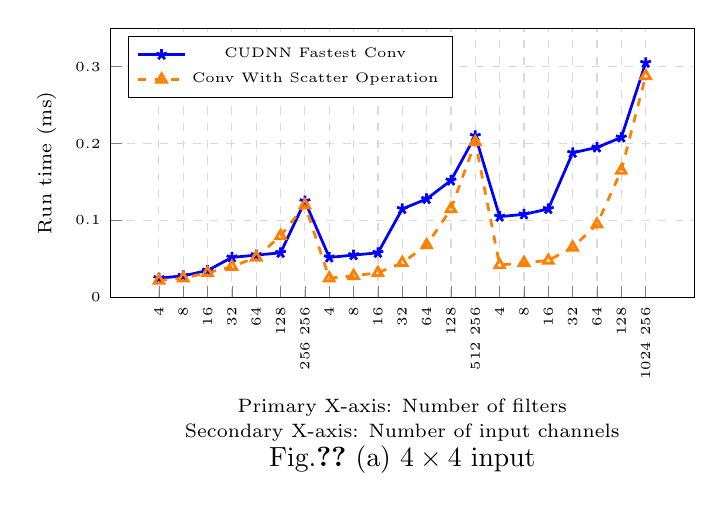
\begin{tikzpicture}
\begin{axis}[
width=9cm,
height=5cm,
xlabel={\shortstack{Primary X-axis: Number of filters \\ Secondary X-axis: Number of input channels}},
xlabel style={font=\scriptsize},
ylabel={Run time (ms)},
ylabel style={font=\scriptsize},
%title={Input size = 4},
%title style={font=\large},
% Primary x-axis (filter numbers)
xtick={1,6,11,16,21,26,31,36,41,46,51,56,61,66,71,76,81,86,91,96,101},
xticklabels={4,8,16,32,64,128,{256\\~256},{4},{8},{16},{32},{64},{128},{512\\~256},{4},{8},{16},{32},{64},{128},{1024\\~256}},
x tick label style={font=\tiny, rotate=90},
y tick label style={font=\tiny},
% Spacing and appearance
ymin=0,
ymax=0.35,
legend pos=north west,
legend style={font=\tiny},
% Remove top tick marks
xtick pos=bottom,
ytick pos=left,
grid=major,
grid style={dashed,gray!30},
]

% CUDNN Fastest Conv (blue line with stars)
\addplot[
color=blue,
mark=star,
mark size=2pt,
line width=1.0pt,
mark options={solid, fill=blue!70}
] coordinates {
(1,0.025) (6,0.028) (11,0.035) (16,0.052) (21,0.055) (26,0.058) (31,0.125)
(36,0.052) (41,0.055) (46,0.058) (51,0.115) (56,0.128) (61,0.152) (66,0.210)
(71,0.105) (76,0.108) (81,0.115) (86,0.188) (91,0.195) (96,0.208) (101,0.305)
};

% Conv With Scatter Operation (orange line with triangles)
\addplot[
color=orange,
mark=triangle,
mark size=2pt,
dashed,
line width=1.0pt,
mark options={solid, fill=orange!70}
] coordinates {
(1,0.022) (6,0.025) (11,0.032) (16,0.040) (21,0.052) (26,0.080) (31,0.120)
(36,0.025) (41,0.028) (46,0.032) (51,0.045) (56,0.068) (61,0.115) (66,0.202)
(71,0.042) (76,0.045) (81,0.048) (86,0.065) (91,0.095) (96,0.165) (101,0.288)
};

\legend{CUDNN Fastest Conv, Conv With Scatter Operation}

\end{axis}
\node[below=50pt] at (current axis.south) {\normalsize Fig.\ref{fig:performance} (a) $4\times4$ input};
\end{tikzpicture}
}
\vspace{0.4cm}  % Add vertical space here



\centerline{
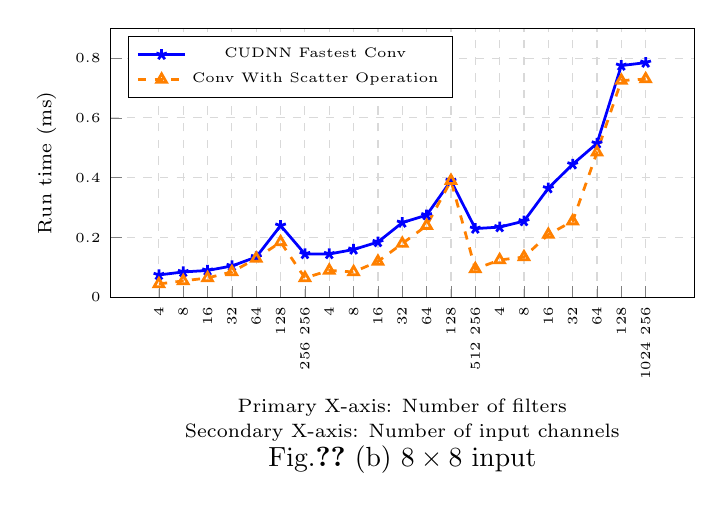
\begin{tikzpicture}
\begin{axis}[
width=9cm,
height=5cm,
xlabel={\shortstack{Primary X-axis: Number of filters \\ Secondary X-axis: Number of input channels}},
xlabel style={font=\scriptsize},
ylabel={Run time (ms)},
ylabel style={font=\scriptsize},
%title={Input size = 4},
%title style={font=\large},
% Primary x-axis (filter numbers)
xtick={1,6,11,16,21,26,31,36,41,46,51,56,61,66,71,76,81,86,91,96,101},
xticklabels={4,8,16,32,64,128,{256\\~256},{4},{8},{16},{32},{64},{128},{512\\~256},{4},{8},{16},{32},{64},{128},{1024\\~256}},
x tick label style={font=\tiny, rotate=90},
y tick label style={font=\tiny},
% Spacing and appearance
ymin=0,
ymax=0.9,
legend pos=north west,
legend style={font=\tiny},
% Remove top tick marks
xtick pos=bottom,
ytick pos=left,
grid=major,
grid style={dashed,gray!30},
]

% CUDNN Fastest Conv (blue line with stars)
\addplot[
color=blue,
mark=star,
mark size=2pt,
line width=1.0pt,
mark options={solid, fill=blue!70}
] coordinates {
(1,0.075) (6,0.085) (11,0.090) (16,0.105) (21,0.135) (26,0.240) (31,0.145)
(36,0.145) (41,0.160) (46,0.185) (51,0.250) (56,0.275) (61,0.390) (66,0.230)
(71,0.235) (76,0.255) (81,0.365) (86,0.445) (91,0.515) (96,0.775) (101,0.785)
};

% Conv With Scatter Operation (orange line with triangles)
\addplot[
color=orange,
mark=triangle,
mark size=2pt,
dashed,
line width=1.0pt,
mark options={solid, fill=orange!70}
] coordinates {
(1,0.045) (6,0.055) (11,0.065) (16,0.085) (21,0.130) (26,0.185) (31,0.065)
(36,0.090) (41,0.085) (46,0.120) (51,0.180) (56,0.240) (61,0.390) (66,0.095)
(71,0.125) (76,0.135) (81,0.210) (86,0.255) (91,0.485) (96,0.725) (101,0.730)
};

\legend{CUDNN Fastest Conv, Conv With Scatter Operation}

\end{axis}
\node[below=50pt] at (current axis.south) {\normalsize Fig.\ref{fig:performance} (b) $8\times8$ input};
\end{tikzpicture}
}
\vspace{0.4cm}  % Add vertical space here


\centerline{
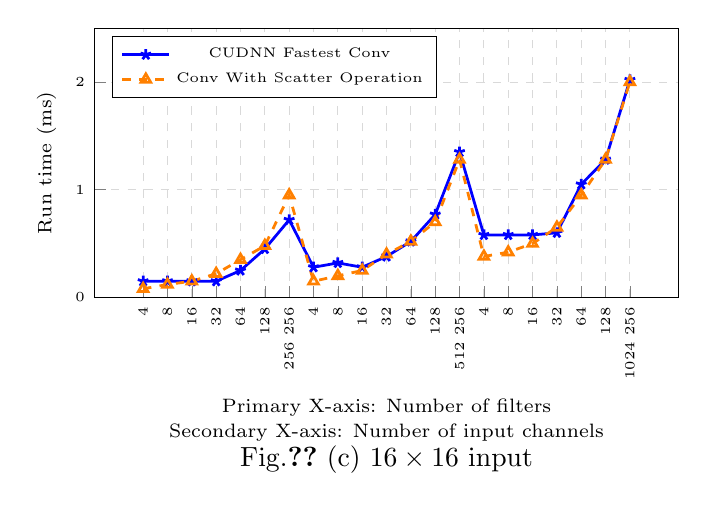
\begin{tikzpicture}
\begin{axis}[
width=9cm,
height=5cm,
xlabel={\shortstack{Primary X-axis: Number of filters \\ Secondary X-axis: Number of input channels}},
xlabel style={font=\scriptsize},
ylabel={Run time (ms)},
ylabel style={font=\scriptsize},
%title={Input size = 4},
%title style={font=\large},
% Primary x-axis (filter numbers)
xtick={1,6,11,16,21,26,31,36,41,46,51,56,61,66,71,76,81,86,91,96,101},
xticklabels={4,8,16,32,64,128,{256\\~256},{4},{8},{16},{32},{64},{128},{512\\~256},{4},{8},{16},{32},{64},{128},{1024\\~256}},
x tick label style={font=\tiny, rotate=90},
y tick label style={font=\tiny},
% Spacing and appearance
ymin=0,
ymax=2.5,
legend pos=north west,
legend style={font=\tiny},
% Remove top tick marks
xtick pos=bottom,
ytick pos=left,
grid=major,
grid style={dashed,gray!30},
]

% CUDNN Fastest Conv (blue line with stars)
\addplot[
color=blue,
mark=star,
mark size=2pt,
line width=1.0pt,
mark options={solid, fill=blue!70}
] coordinates {
(1,0.15) (6,0.15) (11,0.15) (16,0.15) (21,0.25) (26,0.45) (31,0.72)
(36,0.28) (41,0.32) (46,0.28) (51,0.38) (56,0.52) (61,0.77) (66,1.35)
(71,0.58) (76,0.58) (81,0.58) (86,0.60) (91,1.05) (96,1.28) (101,2.02)
};

% Conv With Scatter Operation (orange line with triangles)
\addplot[
color=orange,
mark=triangle,
mark size=2pt,
dashed,
line width=1.0pt,
mark options={solid, fill=orange!70}
] coordinates {
(1,0.08) (6,0.12) (11,0.15) (16,0.22) (21,0.35) (26,0.48) (31,0.95)
(36,0.15) (41,0.20) (46,0.25) (51,0.40) (56,0.52) (61,0.70) (66,1.28)
(71,0.38) (76,0.42) (81,0.50) (86,0.65) (91,0.95) (96,1.28) (101,2.00)
};

\legend{CUDNN Fastest Conv, Conv With Scatter Operation}

\end{axis}
\node[below=50pt] at (current axis.south) {\normalsize Fig.\ref{fig:performance} (c) $16\times16$ input};
\end{tikzpicture}
}
\vspace{0.4cm}  % Add vertical space here



\centerline{
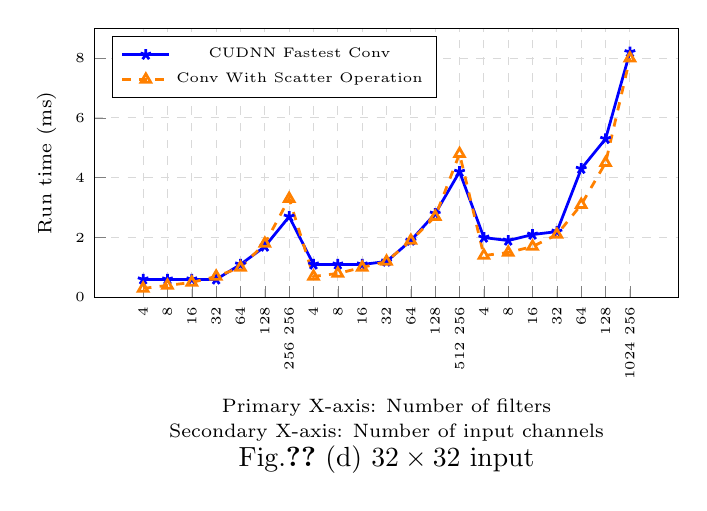
\begin{tikzpicture}
\begin{axis}[
width=9cm,
height=5cm,
xlabel={\shortstack{Primary X-axis: Number of filters \\ Secondary X-axis: Number of input channels}},
xlabel style={font=\scriptsize},
ylabel={Run time (ms)},
ylabel style={font=\scriptsize},
%title={Input size = 4},
%title style={font=\large},
% Primary x-axis (filter numbers)
xtick={1,6,11,16,21,26,31,36,41,46,51,56,61,66,71,76,81,86,91,96,101},
xticklabels={4,8,16,32,64,128,{256\\~256},{4},{8},{16},{32},{64},{128},{512\\~256},{4},{8},{16},{32},{64},{128},{1024\\~256}},
x tick label style={font=\tiny, rotate=90},
y tick label style={font=\tiny},
% Spacing and appearance
ymin=0,
ymax=9,
legend pos=north west,
legend style={font=\tiny},
% Remove top tick marks
xtick pos=bottom,
ytick pos=left,
grid=major,
grid style={dashed,gray!30},
]

% CUDNN Fastest Conv (blue line with stars)
\addplot[
color=blue,
mark=star,
mark size=2pt,
line width=1.0pt,
mark options={solid, fill=blue!70}
] coordinates {
(1,0.6) (6,0.6) (11,0.6) (16,0.6) (21,1.1) (26,1.7) (31,2.7)
(36,1.1) (41,1.1) (46,1.1) (51,1.2) (56,1.9) (61,2.8) (66,4.2)
(71,2.0) (76,1.9) (81,2.1) (86,2.2) (91,4.3) (96,5.3) (101,8.2)
};

% Conv With Scatter Operation (orange line with triangles)
\addplot[
color=orange,
mark=triangle,
mark size=2pt,
dashed,
line width=1.0pt,
mark options={solid, fill=orange!70}
] coordinates {
(1,0.3) (6,0.4) (11,0.5) (16,0.7) (21,1.0) (26,1.8) (31,3.3)
(36,0.7) (41,0.8) (46,1.0) (51,1.2) (56,1.9) (61,2.7) (66,4.8)
(71,1.4) (76,1.5) (81,1.7) (86,2.1) (91,3.1) (96,4.5) (101,8.0)
};

\legend{CUDNN Fastest Conv, Conv With Scatter Operation}

\end{axis}
\node[below=50pt] at (current axis.south) {\normalsize Fig.\ref{fig:performance} (d) $32\times32$ input};
\end{tikzpicture}
}
\vspace{0.4cm}  % Add vertical space here


\centerline{
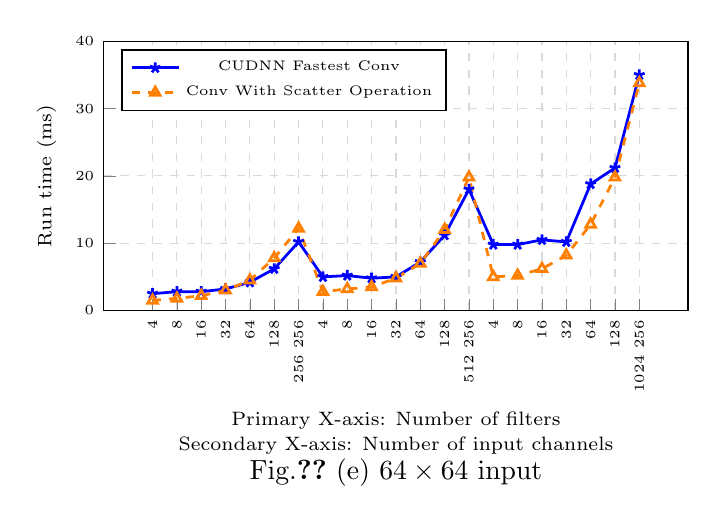
\begin{tikzpicture}
\begin{axis}[
width=9cm,
height=5cm,
xlabel={\shortstack{Primary X-axis: Number of filters \\ Secondary X-axis: Number of input channels}},
xlabel style={font=\scriptsize},
ylabel={Run time (ms)},
ylabel style={font=\scriptsize},
%title={Input size = 4},
%title style={font=\large},
% Primary x-axis (filter numbers)
xtick={1,6,11,16,21,26,31,36,41,46,51,56,61,66,71,76,81,86,91,96,101},
xticklabels={4,8,16,32,64,128,{256\\~256},{4},{8},{16},{32},{64},{128},{512\\~256},{4},{8},{16},{32},{64},{128},{1024\\~256}},
x tick label style={font=\tiny, rotate=90},
y tick label style={font=\tiny},
% Spacing and appearance
ymin=0,
ymax=40,
legend pos=north west,
legend style={font=\tiny},
% Remove top tick marks
xtick pos=bottom,
ytick pos=left,
grid=major,
grid style={dashed,gray!30},
]

% CUDNN Fastest Conv (blue line with stars)
\addplot[
color=blue,
mark=star,
mark size=2pt,
line width=1.0pt,
mark options={solid, fill=blue!70}
] coordinates {
(1,2.5) (6,2.8) (11,2.8) (16,3.2) (21,4.2) (26,6.2) (31,10.2)
(36,5.0) (41,5.2) (46,4.8) (51,5.0) (56,7.2) (61,11.2) (66,18.0)
(71,9.8) (76,9.8) (81,10.5) (86,10.2) (91,18.8) (96,21.2) (101,35.0)
};

% Conv With Scatter Operation (orange line with triangles)
\addplot[
color=orange,
mark=triangle,
mark size=2pt,
dashed,
line width=1.0pt,
mark options={solid, fill=orange!70}
] coordinates {
(1,1.5) (6,1.8) (11,2.2) (16,3.0) (21,4.5) (26,7.8) (31,12.2)
(36,2.8) (41,3.2) (46,3.5) (51,4.8) (56,7.0) (61,12.0) (66,19.8)
(71,5.0) (76,5.2) (81,6.2) (86,8.2) (91,12.8) (96,19.8) (101,33.8)
};

\legend{CUDNN Fastest Conv, Conv With Scatter Operation}

\end{axis}
\node[below=50pt] at (current axis.south) {\normalsize Fig.\ref{fig:performance} (e) $64\times64$ input};
\end{tikzpicture}
}
\vspace{0.4cm}  % Add vertical space here




\centerline{
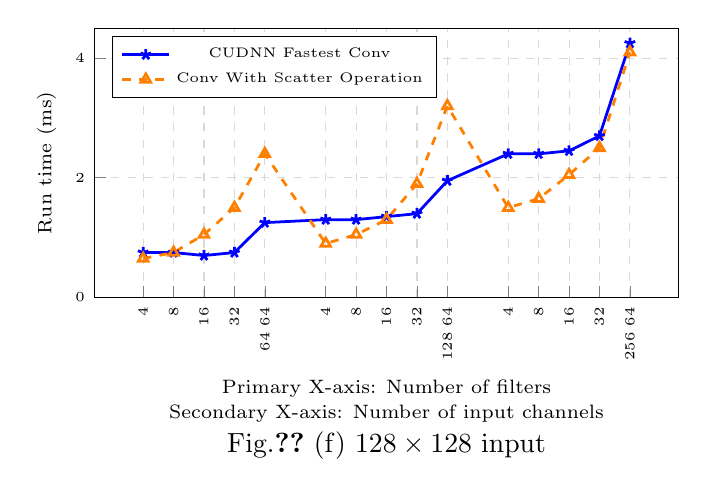
\begin{tikzpicture}
\begin{axis}[
width=9cm,
height=5cm,
xlabel={\shortstack{Primary X-axis: Number of filters \\ Secondary X-axis: Number of input channels}},
xlabel style={font=\scriptsize},
ylabel={Run time (ms)},
ylabel style={font=\scriptsize},
%title={Input size = 4},
%title style={font=\large},
% Primary x-axis (filter numbers) - adjusted for 3 groups of 5 filters each
xtick={1,2,3,4,5,7,8,9,10,11,13,14,15,16,17},
xticklabels={4,8,16,32,{64\\~64},{4},{8},{16},{32},{128\\~64},{4},{8},{16},{32},{256\\~64}},
x tick label style={font=\tiny, rotate=90},
y tick label style={font=\tiny},
% Spacing and appearance
ymin=0,
ymax=4.5,
legend pos=north west,
legend style={font=\tiny},
% Remove top tick marks
xtick pos=bottom,
ytick pos=left,
grid=major,
grid style={dashed,gray!30},
]

% CUDNN Fastest Conv (blue line with stars)
\addplot[
color=blue,
mark=star,
mark size=2pt,
line width=1.0pt,
mark options={solid, fill=blue!70}
] coordinates {
(1,0.75) (2,0.75) (3,0.7) (4,0.75) (5,1.25)
(7,1.3) (8,1.3) (9,1.35) (10,1.4) (11,1.95)
(13,2.4) (14,2.4) (15,2.45) (16,2.7) (17,4.25)
};

% Conv With Scatter Operation (orange line with triangles)
\addplot[
color=orange,
mark=triangle,
mark size=2pt,
dashed,
line width=1.0pt,
mark options={solid, fill=orange!70}
] coordinates {
(1,0.65) (2,0.75) (3,1.05) (4,1.5) (5,2.4)
(7,0.9) (8,1.05) (9,1.3) (10,1.9) (11,3.2)
(13,1.5) (14,1.65) (15,2.05) (16,2.5) (17,4.1)
};

\legend{CUDNN Fastest Conv, Conv With Scatter Operation}

\end{axis}
\node[below=45pt] at (current axis.south) {\normalsize Fig.\ref{fig:performance} (f) $128\times128$ input};
\end{tikzpicture}
}



\begin{figure}[htbp]
\centering
%\centerline{
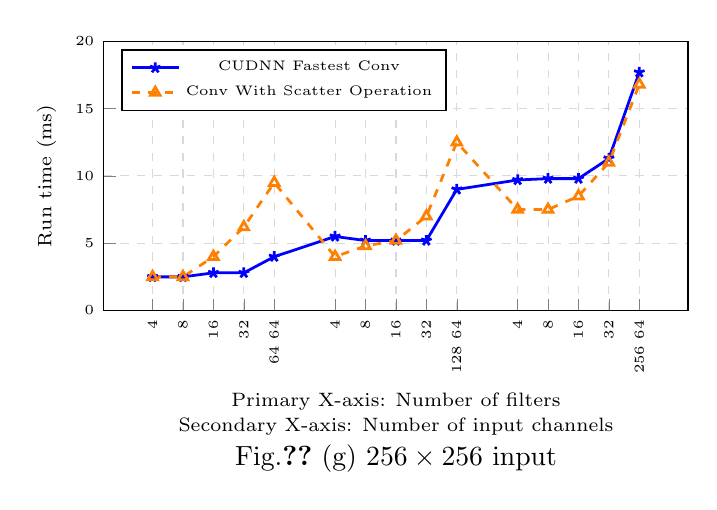
\begin{tikzpicture}
\begin{axis}[
width=9cm,
height=5cm,
xlabel={\shortstack{Primary X-axis: Number of filters \\ Secondary X-axis: Number of input channels}},
xlabel style={font=\scriptsize},
ylabel={Run time (ms)},
ylabel style={font=\scriptsize},
%title={Input size = 4},
%title style={font=\large},
% Primary x-axis (filter numbers) - adjusted for 3 groups of 5 filters each
xtick={1,2,3,4,5,7,8,9,10,11,13,14,15,16,17},
xticklabels={4, 8, 16, 32, \rotatebox{90}{\rotatebox{-90}{\shortstack{64  64}}}, 4, 8, 16, 32, \rotatebox{90}{\rotatebox{-90}{\shortstack{128  64}}}, 4, 8, 16, 32, \rotatebox{90}{\rotatebox{-90}{\shortstack{256  64}}}},
x tick label style={font=\tiny, rotate=90},
y tick label style={font=\tiny},
% Spacing and appearance
ymin=0,
ymax=20,
legend pos=north west,
legend style={font=\tiny},
% Remove top tick marks
xtick pos=bottom,
ytick pos=left,
grid=major,
grid style={dashed,gray!30},
]

% CUDNN Fastest Conv (blue line with stars)
\addplot[
color=blue,
mark=star,
mark size=2pt,
line width=1.0pt,
mark options={solid, fill=blue!70}
] coordinates {
(1,2.5) (2,2.5) (3,2.8) (4,2.8) (5,4.0)
(7,5.5) (8,5.2) (9,5.2) (10,5.2) (11,9.0)
(13,9.7) (14,9.8) (15,9.8) (16,11.3) (17,17.7)
};

% Conv With Scatter Operation (orange line with triangles)
\addplot[
color=orange,
mark=triangle,
mark size=2pt,
dashed,
line width=1.0pt,
mark options={solid, fill=orange!70}
] coordinates {
(1,2.5) (2,2.5) (3,4.0) (4,6.2) (5,9.5)
(7,4.0) (8,4.8) (9,5.2) (10,7.0) (11,12.5)
(13,7.5) (14,7.5) (15,8.5) (16,11.0) (17,16.8)
};

\legend{CUDNN Fastest Conv, Conv With Scatter Operation}

\end{axis}
\node[below=45pt] at (current axis.south) {\normalsize Fig.\ref{fig:performance}  (g) $256\times256$ input};
\end{tikzpicture}
%}
\caption{Performance comparison of cuDNN (blue) and
the proposed scatter convolution (orange) across seven
input resolutions.}
\label{fig:performance}
\end{figure}


NVIDIA's cuDNN offers eight distinct forward-convolution
implementations, and for every experiment we measure the fastest of
those eight via cuDNN's autotuner. As shown in Fig.\ref{fig:performance} (a)-(g),
across the seven plots (input sizes $4 \to 256$) our
scatter-based kernel still dominates that ``best-of-eight'' cuDNN
baseline in the majority of layer configurations. Counting every
(resolution $\times$ input-channel $\times$ filter) triplet, the scatter
variant is quicker in most cases, with typical speed-ups of
$1.1\times$--$1.6\times$ and a peak of $\approx 2\times$ for the very
small $4\times4$ activations. The gain is most pronounced whenever the
spatial footprint is modest ($\le 32\times32$) or the channel--filter
product is under $\sim16\text{\,K}$, where kernel-launch latency and
global-memory traffic dominate the cost of convolution; the single-pass
scatter design removes the data-lowering staging step and sustains
higher memory-bandwidth utilisation in that regime. As the resolution
grows beyond $64\times64$ and the workload becomes compute-bound,
cuDNN paths occasionally pull ahead, yet even at
$256\times256$ our kernel still wins for 4 of the 9 channel--filter
pairs tested. In practice, this means the scatter kernel is the better
choice for mid‑to‑deep layers where spatial dimensions have shrunk and channel depth has increased, while cuDNN
remains preferable only for the first one or two encoder layers of very
high-resolution networks.



%\begin{figure}[htbp]            % htbp gives LaTeX more freedom
%  \centering
%  \includegraphics[width=0.47\textwidth]{fig/FL_timing/fig-conv-performance/size_4.png}
%  \caption{Performance of the two convolution variants (input size $4\times4$).}
%  \label{fig:1}
%\end{figure}
%
%
%\begin{figure}[htbp]            % htbp gives LaTeX more freedom
%  \centering
%  \includegraphics[width=0.47\textwidth]{fig/FL_timing/fig-conv-performance/size_8.png}
%  \caption{Performance of the two convolution variants (input size $8\times8$).}
%  \label{fig:2}
%\end{figure}
%
%
%\begin{figure}[htbp]            % htbp gives LaTeX more freedom
%  \centering
%  \includegraphics[width=0.47\textwidth]{fig/FL_timing/fig-conv-performance/size_16.png}
%  \caption{Performance of the two convolution variants (input size $16\times16$).}
%  \label{fig:3}
%\end{figure}
%
%\begin{figure}[htbp]            % htbp gives LaTeX more freedom
%  \centering
%  \includegraphics[width=0.47\textwidth]{fig/FL_timing/fig-conv-performance/size_32.png}
%  \caption{Performance of the two convolution variants (input size $32\times32$).}
%  \label{fig:4}
%\end{figure}
%
%\begin{figure}[htbp]            % htbp gives LaTeX more freedom
%  \centering
%  \includegraphics[width=0.47\textwidth]{fig/FL_timing/fig-conv-performance/size_64.png}
%  \caption{Performance of the two convolution variants (input size $64\times64$).}
%  \label{fig:5}
%\end{figure}
%
%\begin{figure}[htbp]            % htbp gives LaTeX more freedom
%  \centering
%  \includegraphics[width=0.47\textwidth]{fig/FL_timing/fig-conv-performance/size_128.png}
%  \caption{Performance of the two convolution variants (input size $128\times128$).}
%  \label{fig:6}
%\end{figure}
%
%\begin{figure}[htbp]            % htbp gives LaTeX more freedom
%  \centering
%  \includegraphics[width=0.47\textwidth]{fig/FL_timing/fig-conv-performance/size_256.png}
%  \caption{Performance of the two convolution variants (input size $256\times256$).}
%  \label{fig:7}
%\end{figure}



%% ---------- first panel (starts Figure N) ----------
%\begin{figure}[htbp]
%  \centering
%  \includegraphics[width=0.45\textwidth]{fig/FL_timing/fig-conv-performance/size_4.png}
%  \caption{(a) $4\times4$ input}
%  \label{fig:conv-perf:4}
%\end{figure}
%
%% ---------- second panel — same Figure N  ----------
%\begin{figure}[htbp]
%  \ContinuedFloat          % keep Figure N, add (b)
%  \centering
%  \includegraphics[width=0.45\textwidth]{fig/FL_timing/fig-conv-performance/size_8.png}
%  \caption{(b) $8\times8$ input}
%  \label{fig:conv-perf:8}
%\end{figure}
%
%% ---------- third panel ----------
%\begin{figure}[htbp]
%  \ContinuedFloat
%  \centering
%  \includegraphics[width=0.45\textwidth]{fig/FL_timing/fig-conv-performance/size_16.png}
%  \caption{(c) $16\times16$ input}
%  \label{fig:conv-perf:16}
%\end{figure}
%
%% ---------- keep repeating the pattern ----------
%\begin{figure}[htbp]
%  \ContinuedFloat
%  \centering
%  \includegraphics[width=0.45\textwidth]{fig/FL_timing/fig-conv-performance/size_32.png}
%  \caption{(d) $32\times32$ input}
%  \label{fig:conv-perf:32}
%\end{figure}
%
%\begin{figure}[htbp]
%  \ContinuedFloat
%  \centering
%  \includegraphics[width=0.45\textwidth]{fig/FL_timing/fig-conv-performance/size_64.png}
%  \caption{(e) $64\times64$ input}
%  \label{fig:conv-perf:64}
%\end{figure}
%
%\begin{figure}[htbp]
%  \ContinuedFloat
%  \centering
%  \includegraphics[width=0.45\textwidth]{fig/FL_timing/fig-conv-performance/size_128.png}
%  \caption{(f) $128\times128$ input}
%  \label{fig:conv-perf:128}
%\end{figure}
%
%\begin{figure}[htbp]
%  \ContinuedFloat
%  \centering
%  \includegraphics[width=0.45\textwidth]{fig/FL_timing/fig-conv-performance/size_256.png}
%  \caption{(g) $256\times256$ input\\[4pt]
%           \textbf{Figure \ref{fig:conv-perf:4}}\,. Performance comparison of cuDNN (blue) and the proposed scatter convolution (orange) across seven input resolutions.}
%  \label{fig:conv-perf:256}
%\end{figure}

%\centerline{
%\begin{tikzpicture}
%\begin{axis}[
%ybar,
%width=9cm,
%height=5cm,
%ylabel={Run time (ms)},
%title={Input size = 4},
%title style={font=\large},
%% Primary x-axis (filter numbers)
%xtick={1,6,11,16,21,26,31,36,41,46,51,56,61,66,71,76,81,86,91,96,101},
%xticklabels={4,8,16,32,64,128,{256\\~256},{4},{8},{16},{32},{64},{128},{512\\256},{4},{8},{16},{32},{64},{128},{1024\\256}},
%x tick label style={font=\tiny, rotate=90},
%% Spacing and appearance
%bar width=0.22cm,
%bar shift=0pt,
%ymin=0,
%ymax=0.35,
%legend pos=north west,
%legend style={font=\tiny},
%legend image code/.code={
%\draw[#1] (0cm,-0.1cm) rectangle (0.3cm,0.1cm);
%},
%% Add vertical lines to separate groups
%% Remove top tick marks
%xtick pos=bottom,
%ytick pos=left,
%]
%
%% CUDNN Fastest Conv (blue bars)
%\addplot[fill=blue!70, area legend, bar shift=-0.15cm] coordinates {
%(0.8,0.025) (5.8,0.028) (10.8,0.035) (15.8,0.052) (20.8,0.055) (25.8,0.058) (30.8,0.125)
%(35.8,0.052) (40.8,0.055) (45.8,0.058) (50.8,0.115) (55.8,0.128) (60.8,0.152) (65.8,0.210)
%(70.8,0.105) (75.8,0.108) (80.8,0.115) (85.8,0.188) (90.8,0.195) (95.8,0.208) (100.8,0.305)
%};
%
%% Conv With Scatter Operation (orange bars)
%\addplot[fill=orange!70, area legend, bar shift=0.15cm] coordinates {
%(1.2,0.022) (6.2,0.025) (11.2,0.032) (16.2,0.040) (21.2,0.052) (26.2,0.080) (31.2,0.120)
%(36.2,0.025) (41.2,0.028) (46.2,0.032) (51.2,0.045) (56.2,0.068) (61.2,0.115) (66.2,0.202)
%(71.2,0.042) (76.2,0.045) (81.2,0.048) (86.2,0.065) (91.2,0.095) (96.2,0.165) (101.2,0.288)
%};
%
%\legend{CUDNN Fastest Conv, Conv With Scatter Operation}
%
%\end{axis}
%\end{tikzpicture}
%}